
\chapter{Preferences over static plans\label{sec:decisiontheory}}
%
%\begin{quote}
%%{\em Events occur with probabilities in inverse ratio to their desirability.}
% {\em The probability of anything happening is in inverse ratio to its desirability.} Murphy's law  as cited by \citet[p.~27]{bucklew2004}.
%\end{quote}
This chapter describes  static representations of five classes of preferences over risky prospects. All  incorporate
{\em risk aversion}, meaning displeasure from
 risks governed by  well known probability distributions.  Two
of them also incorporate  {\em uncertainty aversion}, meaning  dislike of not knowing a  probability distribution.
%The setting is static, but in  section \ref{sec:dynamics_1} we indicate  dynamic settings that are special cases of the static one.
%\index{Murphy's law}%


\section{Basic objects\label{sec:decisiontheory2}}

Basic ingredients are (a) a set of states of the world, (b) plans describing outcomes as functions
of the state of the world, (c) a  utility  function mapping outcomes into utilities, (d) either a probability distribution or a \textit{set\/}
of probability distributions over states of the world; and (e) a way of measuring the discrepancy between two probability distributions.
In this section, we'll use the following.
\begin{itemize}
 \item[a.] There is a  finite set of \underline{states} ${\cal I} = \{i= 1, \ldots, I\}$.
 \item[b.] A (consumption) \underline{plan} is a function $c: {\cal I} \rightarrow {\mathbb R}$.  
 \item[c.] $u: {\mathbb R} \rightarrow {\mathbb R}$ is a \underline{utility function}.
 \item[d.] $\pi$ is an $I \times 1$ vector of nonnegative
\underline{probabilities} over  states, with $\pi_ i \geq 0, \sum_{i=1}^I \pi_i = 1$.
 \item[e.] The \underline{relative entropy} of a probability vector  $\hat \pi$ with respect to a probability vector $\pi$
is the expected value of the logarithm of the  likelihood ratio $m_i \doteq \Bigl( \frac{\hat \pi_i}{\pi_i} \Bigr) $
 under   distribution $\hat \pi$:
\[ \textrm{ent}(\pi, \hat \pi) = \sum_{i=1}^I \hat \pi_i  \log \Bigl( \frac{\hat \pi_i}{\pi_i} \Bigr)   = \sum_{i=1}^I \pi_i \Bigl( \frac{\hat \pi_i}{\pi_i} \Bigr) \log \Bigl( \frac{\hat \pi_i}{\pi_i} \Bigr)   \]
or
 \begin{equation} \label{eqn:def_ent}
    \textrm{ent}(\pi, \hat \pi) = \sum_{i=1}^I \pi_i m_i \log m_i  . \end{equation}
\end{itemize}

% 
% \begin{definition}\label{defn:rel_entropy_baby}
% The \underline{relative entropy} of a probability vector  $\hat \pi$ with respect to a probability vector $\pi$
% is the expected value of the logarithm of the  likelihood ratio $m_i \doteq \Bigl( \frac{\hat \pi_i}{\pi_i} \Bigr) $
%  under   distribution $\hat \pi$:
% \[ \textrm{ent}(\pi, \hat \pi) = \sum_{i=1}^I \hat \pi_i  \log \Bigl( \frac{\hat \pi_i}{\pi_i} \Bigr)   = \sum_{i=1}^I \pi_i \Bigl( \frac{\hat \pi_i}{\pi_i} \Bigr) \log \Bigl( \frac{\hat \pi_i}{\pi_i} \Bigr)   \]
% or
%  \begin{equation} \label{eqn:def_ent}
%     \textrm{ent}(\pi, \hat \pi) = \sum_{i=1}^I \pi_i m_i \log m_i  . \end{equation}
% \end{definition}
\begin{remark}\label{remark1}
The likelihood ratio $m_i$ is a discrete random variable.
For any discrete random variable $\{x_i\}_{i=1}^I$, the expected  value under the $\hat \pi_i$ distribution can
be represented as the expected  value of  $x_i$ times the `shock'  $m_i$ under the $\pi$ distribution:
\[ \hat E x = \sum_{i=1}^I x_i \hat \pi_i = \sum_{i=1}^I m_i x_i  \pi_i = E m x ,\]
where $\hat E$ is the mathematical  expectation under the $\hat \pi$ distribution and $E$ is the
expectation under the $\pi$ distribution.
\end{remark}

\noindent Evidently,
\[ \hat E 1 = E m = 1\]
and relative entropy is
\[ E m \log m  = \hat E \log m .\]

 Figure \ref{fig_entropy_I2} depicts
 entropy as a function of $\hat \pi_1$ when $I=2$ and $\pi_1 = .5$.\footnote{When $\pi_1 \in (0,1)$, entropy is finite for both $\hat \pi_1 = 0$
 and $\hat \pi_1 = 1$ because $\lim_{x\rightarrow 0} x \log x = 0$  However, when $\pi_1=0$ or $\pi_1=1$, entropy
 is infinite.}
\begin{figure}[htp]
\centering
\includegraphics[height=2in]{new_figure4.eps}
\caption[Entropy]{Entropy as a function of $\hat \pi_1$ when $\pi_1 = .5$.}\label{fig_entropy_I2}
\end{figure}



\section{Five preference specifications}

We describe five types of preferences over plans.  Types 1, 4, and 5, each of which is cast in terms of a unique probability distribution,
express risk-aversion, but not model  ambiguity aversion.  Our main focus will eventually be on types 2 and 3, each of  which expresses 
aversion to model ambiguity and each of which 
is cast in terms of a set  of probability distributions.  The set of distributions expresses the decision maker's  ambiguity about the probability model.  Minimization over probability distributions expresses his aversion to ambiguity.

\begin{enumerate}
\item\textbf{Expected utility.}
A decision maker is said to have \textit{expected
utility preferences} when he  ranks plans $c$ by  their expected utilities
\[ \sum_{i=1}^I u(c_i) \pi_i,  \]
where $u$ is a  unique utility function and $\pi$ is a  unique probability measure over states.  A known $\pi$ expresses risk.  Curvature of $u$ expresses risk aversion.

\item\textbf{Constraint preferences.} A decision maker  is said to have \textit{constraint preferences} when he ranks plans $c$ according to
\begin{equation}\label{Pconstraint}  \min_{\{m_i \geq 0\}_{i=1}^I}  \sum_{i=1}^I m_i\pi_i  u(c_i) \end{equation}
 subject to
\[\sum_{i=1}^I \pi_i m_i \log m_i \leq \eta \]
and
\[ \sum_{i=1}^I \pi_i m_i = 1 .\]
Here $\eta \geq 0$ defines an entropy ball of probability distributions $\hat \pi = m \pi$ surrounding
a baseline distribution $\pi$. From remark \ref{remark1},
$  \sum_{i=1}^I m_i\pi_i  u(c_i) $ is the expected value of $u(c)$ under a twisted  probability distribution $\{\hat \pi_i\}_{i=1}^I = \{m_i \pi_i\}_{i=1}^I$. Larger values of the entropy constraint $\eta$
 indicate more apprehension about the probability distribution $\{\pi_i\}_{i=1}^I$.

We call  minimization problem \eqref{Pconstraint} a \textit{constraint problem}. To find
 the minimizing probabilities, we  form the
Lagrangian
\begin{equation}\label{eqn:constraint_Lagrangian}
L = \sum_{i=1}^I m_i \pi_i u(c_i) +  \tilde \theta\bigl[\sum_{i=1}^I \pi_i m_i \log m_i - \eta \bigr]
\end{equation}
where $\tilde \theta \geq 0$ is a Lagrange multiplier associated with the entropy constraint.  Subject to the additional constraint that
$\sum_{i=1}^I m_i  \pi_i =1$, we want to  minimize \eqref{eqn:constraint_Lagrangian}
with respect to $\{m_i\}_{i=1}^I$ and to maximize it with respect to $\tilde \theta$.
The minimizing probability distortions (likelihood ratios) are %Minimizing the expression given by \eqref{eqn:constraint_Lagrangian} gives
 \begin{equation}\label{eqn:Murphys_law_2} \tilde m_i(c;\tilde \theta) 
 = \frac{ \exp \bigl(- u(c_i)/\tilde \theta\bigr)}{\sum_j \pi_j \exp \bigl(- u(c_j)/\tilde \theta\bigr) } .\end{equation}
  
 To compute the Lagrange multiplier $\tilde \theta(c, \eta)$, we must solve
\[ \sum_i \pi_i \tilde m_i (c;\tilde \theta ) \log (\tilde m_i (c;\tilde \theta ))  = \eta \]
or
\begin{equation}\label{eqn:entropy_grand}
\sum_i \pi_i \frac{ \exp \bigl(- u(c_i)/\tilde \theta\bigr)}{\sum_j \pi_j \exp \bigl(- u(c_j)/\tilde \theta\bigr) }
\log \biggl[\frac{ \exp \bigl(- u(c_i)/\tilde \theta\bigr)}{\sum_j \pi_j \exp \bigl(- u(c_j)/\tilde \theta\bigr) }
\biggr] = \eta \end{equation}
for $\tilde \theta = \tilde \theta(c; \eta)$.  For a fixed $\eta$, the $\tilde \theta$ that solves this equation is evidently
a function of the consumption plan $c$. With $\tilde \theta(c;\eta)$ in hand we can
obtain worst-case probabilities as functions $ \pi_i\tilde m_i(c;\eta)$ of $\eta$.
% 
% At a given allocation, the Lagrange multiplier $\tilde \theta$ associated with  the entropy constraint for  constraint preferences
% is a function of $\eta$.
%  To solve for $\tilde \theta$ as a function of $\eta$ and the allocation $c$, substitute formula \eqref{eqn:Murphys_law_2} for the minimizing $\hat m_i$  into
%  the entropy constraint at equality  to obtain
% \begin{equation}\label{eqn:entropy_grand}
% \sum_i \pi_i \frac{ \exp \bigl(- u(c_i)/\tilde \theta\bigr)}{\sum_j \pi_j \exp \bigl(- u(c_j)/\tilde \theta\bigr) }
% \log \biggl[\frac{ \exp \bigl(- u(c_i)/\tilde \theta\bigr)}{\sum_j \pi_j \exp \bigl(- u(c_j)/\tilde \theta\bigr) }
% \biggr] = \eta .\end{equation}

% By virtue of a complementary slackness condition,
The indirect (expected) utility function under constraint
preferences is
\begin{equation}\label{eq:indirect_constraint}
\sum_{i=1}^I   \pi_i \tilde m_i(c_i;\eta) u(c_i) = \sum_{i=1}^I  \pi_i \left[\frac{\exp(-\tilde \theta^{-1} u(c_i))}
  {\sum_{j=1}^I \exp(-\tilde \theta^{-1} u(c_j) ) \pi_j } \right]    u(c_i) .
\end{equation}
Entropy evaluated at the minimizing probability distortion   \eqref{eqn:Murphys_law_2} equals $E \tilde m \log \tilde m$  or
\begin{eqnarray}\label{eqn:entropy_constraint}
& & \sum_{i=1}^I   \left[\frac{\exp(-\tilde \theta^{-1} u(c_i))}
  {\sum_{j=1}^I \exp(-\tilde \theta^{-1} u(c_j) ) \pi_j } \right]  \times \cr
   & & \left\{ -\tilde \theta^{-1} u(c_i) + \log \left(\sum_{j=1}^I \exp(-\tilde \theta^{-1} u(c_j) ) \pi_j \right)
     \right\}  \pi_i \cr
  & = & -\tilde \theta^{-1} \sum_{i=1}^I  \pi_i \left[\frac{\exp(-\tilde \theta^{-1} u(c_i))}
  {\sum_{j=1}^I \exp(-\tilde \theta^{-1} u(c_j) ) \pi_j } \right]    u(c_i)  \cr
  & & + \log \left(\sum_{j=1}^I \exp(-\tilde \theta^{-1} u(c_j) ) \pi_j \right) .
     \end{eqnarray}
Expression \eqref{eqn:entropy_constraint} implies that
\begin{eqnarray}
 - \tilde \theta \log \left(\sum_{j=1}^I \exp(-\tilde \theta^{-1} u(c_j) ) \pi_j \right)  & = &
  \sum_{i=1}^I  \pi_i \left[\frac{\exp(-\tilde \theta^{-1} u(c_i))}
  {\sum_{j=1}^I \exp(-\tilde \theta^{-1} u(c_j) ) \pi_j } \right]    u(c_i) \cr
  & + &  \tilde \theta (c;\eta) \sum_{i=1}^I \log \tilde m_i(c;\eta) \tilde m_i(c;\eta) \pi_i ,
\end{eqnarray}
where the last term  is $\tilde \theta$ times the entropy of the worst-case probability distribution.   
% 
% 
% 
% $\tilde \theta$ times entropy under the worst-case model equals
% minus expected utility under the worst-case model plus the expression
% \[  - \tilde \theta \log \left(\sum_{j=1}^I \exp(-\tilde \theta^{-1} u(c_j) ) \pi_j \right) .\]
We shall encounter a closely related  expression  soon.
%where $ \tilde m_i(c_i;\eta) \pi_i$ is the worst-case probability for state $i$.

\item\textbf{Multiplier preferences.}  A decision maker is said to have \textit{multiplier preferences} when he ranks consumption plans $c$
according to
\begin{equation}\label{Pmultiplier}
{\sf T}u(c) \doteq \min_{\{m_i \geq 0\}_{i=1}^I}  \sum_{i=1}^I \pi_i m_i [  u(c_i) + \theta \log m_i ] \end{equation}
subject to
\[ \sum_{i=1}^I \pi_i m_i = 1 .\]
Here $\theta \in (\underline \theta, +\infty )$ is a  `penalty parameter' that governs a `cost' to an `evil agent' who distorts probabilities by
 choosing $\{m_i\}_{i=1}^I$.  %This minimization is intended to  express the maximizing decision maker's concern about possible misspecification of the baseline model $\pi$.
 Lower
values of the penalty parameter $\theta$ express more apprehension about  the baseline probability distribution $\pi$.\footnote{See
\citet{CMMM2008} for axioms that justify  constraint and multiplier preferences.}
We call the minimization problem  on the right side of \eqref{Pmultiplier}   a \textit{multiplier problem}. 
The minimizing probability that solves  the multiplier problem  is
 \begin{equation}\label{eqn:Murphys_law} \hat m_i(c; \theta) = \frac{ \exp \bigl(- u(c_i)/\theta\bigr)}{\sum_j \pi_j \exp \bigl(- u(c_j)/\theta\bigr) } .\end{equation}
 We can  solve
\begin{equation}\label{eqn:entropy_grand_2}
\sum_i \pi_i \frac{ \exp \bigl(- u(c_i)/ \theta\bigr)}{\sum_j \pi_j \exp \bigl(- u(c_j)/ \theta\bigr) }
\log \biggl[\frac{ \exp \bigl(- u(c_i)/\theta\bigr)}{\sum_j \pi_j \exp \bigl(- u(c_j)/\theta\bigr) }
\biggr] = \tilde \eta  \end{equation} to find an entropy level $\tilde \eta (c; \theta)$  associated with multiplier preferences
with penalty parameter $\theta$ and allocation $c$.
For a fixed $\theta$, the $\tilde \eta$ that solves this equation is a function of the consumption
plan $c$
\begin{remark}
The forms of  \eqref{eqn:Murphys_law_2} and \eqref{eqn:Murphys_law} are identical, but the Lagrange multiplier $\tilde \theta$
 appears in \eqref{eqn:Murphys_law_2} while the penalty parameter or multiplier $\theta$ appears in \eqref{eqn:Murphys_law} . % is the presence of the Lagrange multiplier $\tilde \theta$
%versus the penalty parameter $\theta$.
\end{remark}

\begin{remark}
Formulas \eqref{eqn:Murphys_law_2} and \eqref{eqn:Murphys_law} show that worst-case probabilities are
\textit{context specific} in the sense that they depend both on the utility function $u$ and the consumption plan $c$.
\end{remark}

\begin{remark} If we add $\theta $ times entropy under the worst-case model to expected utility under the worst-case model,
we find that the indirect utility function function under multiplier preferences is
\[  -  \theta \log \left(\sum_{j=1}^I \exp(- \theta^{-1} u(c_j) ) \pi_j \right) .\]

\end{remark}

\item\textbf{Risk-sensitive preferences.}
%
% attains    $\min_{\{m_i \geq 0\}_{i=1}^I}  \sum_{i=1}^I \pi_i m_i [  u(c_i) + \theta \log m_i ]$, subject to
%$ \sum_{i=1}^I \pi_i m_i = 1 $.
 Substituting $\hat m_i$ into $\sum_{i=1}^I \pi_i \hat m_i [  u(c_i) + \theta \log \hat m_i ]$  gives the indirect utility function
\begin{equation}\label{eqn:risksensitive} {\sf T} u(c) \doteq - \theta \log \sum_{i=1}^I \pi_i \exp\bigl(- u(c_i)/\theta  \bigr). \end{equation}
%and ${\sf T} u(c) =\sum_{i=1}^I \pi_i \hat m_i [  u(c_i) + \theta \log \hat m_i ]$.
 Here  ${\sf T} u$  in \eqref{eqn:risksensitive} is  the \textit{risk-sensitivity} operator of \citet{jacobson} and \citet{whittle}.
% ${\sf T} u(c)$
 It  defines  a {\em risk-sensitive}  preference ordering over plans $c$.  Because it is not linear
in utilities $u(c_i)$ and probabilities $\pi_i$, it is said not to be separable across states.
Because risk-sensitive preferences use a unique probability distribution, they apparently  express no model distrust or ambiguity. Instead, they
make an additional adjustment for risk-aversion beyond that embedded in the curvature
of $u$.
For  $I=2, c_1=2, c_2=1$, $u(c) = \ln c$,  figure \ref{fig_new_figure3} plots the risk-sensitive criterion ${\sf T} u(c)$ defined in  \eqref{eqn:risksensitive}
 as a function of $\pi_1$  for values of $\theta$
 of 100 and .6. For large values of $\theta$,  ${\sf T} u(c)$ is approximately linear in the  probability $\pi_1$, but for lower values of $\theta$,
 ${\sf T} u(c)$ has considerable curvature as a function of $\pi_1$. (Under  expected utility, i.e.,
$\theta =+\infty $,  ${\sf T}u(c)$ is linear in $\pi_1$, but  it is convex as a function of $\pi_1$ when $\theta< + \infty$.)


\begin{figure}[htp]
\centering
\includegraphics[height=2in]{new_figure3.eps}
\caption[${\sf T} u(c)$]{${\sf T} u(c)$ as a function of $\pi_1$ for $\theta=100$ (nearly linear line) and $\theta=.6$ (convex curved line). Here $I=2, c_1=2, c_2=1$, $u(c) = \ln c$.}\label{fig_new_figure3}
\end{figure}


\item\textbf{Ex post Bayesian preferences.} A decision maker is said to have {\em ex post Bayesian preferences}
when he ranks consumption plans according to
the expected utility function
\[ \sum_i \hat \pi_i (c^*) u(c_i) \]
where  $\hat \pi(c^*)$ is the   worst-case probability distribution associated with multiplier or constraint preferences
evaluated at a particular consumption plan $c^* = \{c_i^*\}_{i=1}^I$.
 At
 $c^*$, an ex post Bayesian's indifference curves are  tangent to those for  multiplier and constraint preferences with appropriately chosen
$\theta$ and $\eta$, respectively.



 \end{enumerate}



\begin{remark}\label{rem:moment_generate}
In \eqref{eqn:risksensitive}, % that defines $ {\sf T} u(c)$,
 $E \exp\bigl(-u(c_i)/\theta\bigr) = \sum_{i=1}^I \pi_i \exp\bigl(- u(c_i)/\theta  \bigr) $ is evidently
a {\em moment generating function} for the random variable $u(c_i)$, while $ g(\theta^{-1}) \doteq  \log \sum_{i=1}^I \pi_i \exp\bigl(- u(c_i)/\theta  \bigr)$ is a {\em cumulant generating function},
$g(\theta^{-1}) = \sum_{j=1}^\infty \kappa_j \frac{{(-\theta^{-1})}^{j}}{j!}$, where $\kappa_j$ is the $j$th cumulant of the random variable $u(c)$.  Then
${\sf T}u(c) = -\theta g(\theta^{-1}) = -\theta \sum_{j=1}^\infty \kappa_j \frac{{(-\theta^{-1})}^{j}}{j!}$. In general, when $\theta < +\infty$, ${\sf T} u(c)$ depends on cumulants of all orders.  These statements extend to cases with  continuous probability distributions for $c$ and therefore for $u(c)$.
For the particular  case  $u(c) \sim {\mathcal N}(\mu_u, \sigma_u^2)$,
$\kappa_1 = \mu_u, \kappa_2 = \sigma_u^2$ ,and $\kappa_j = 0 \ \forall j \geq 3$, so
${\sf T} u(c) = \mu_u - \frac{1}{2 \theta} \sigma_u^2$, which becomes expected utility $\mu_u$ when $\theta^{-1} = 0$.
\end{remark}

\index{moment generating function}%
\index{cumulant generating function}%
\index{cumulant}%
%
%\section{To be done}
%
%Add comments on relationships among the various types of preferences, playing up the convenience of the connection between risk-sensitivity and robustness.




\section{Comparing  preferences} % and between $\eta$ and $\theta$}

 For the special case in which $I=2$, $c_1=2, c_2=1$, $u(c) = \ln c$,  and  $\pi_1 =.5$, figures \ref{fig_new_figure1} and \ref{fig_new_figure2} depict   the determination of worst-case probabilities under constraint and multiplier preferences, respectively.
Figure \ref{fig_new_figure1} graphs  entropy as a function of $\hat \pi_1$. The figure also plots expected utility under the twisted probability distribution, namely, $\hat E u(c) = u(c_2) + \hat \pi_1 (u(c_1) - u(c_2)) $, which is evidently  a linear function of $\hat \pi_1$.  The entropy constraint $\sum_{i=1}^I \pi_i m_i \log m_i \leq \eta$
implies a convex set $\hat \Pi_1$ of $\hat \pi_1$'s that constrains the malevolent agent who chooses $\hat \pi_1$, namely, the set of  $\hat \pi_1$'s for which
 the entropy curve lies below the horizontal dotted line at an entropy level of $\eta = .25$.  Unless $u(c_1) = u(c_2)$, the $\hat \pi_1$ that minimizes
$ \hat E u(c)$ is at the boundary of the set $\hat \Pi_1$.

 As a function of $\hat \pi_1 = m_1 \pi_1$, figure \ref{fig_new_figure2} shows the function  $ \sum_{i=1}^I \pi_i m_i [  u(c_i) + \theta \log m_i ]$ that is to be minimized in the multiplier problem.  Evidently, from figure \ref{fig_new_figure2} and also from formula \eqref{eqn:Murphys_law}, lower values of $\theta$ lead to lower, and thus more distorted,  minimizing values of $\hat \pi_1$.
The figure  indicates how one can construct a Lagrange  multiplier $\tilde \theta$  associated with a given entropy constraint $\eta$  and a given  consumption plan.  Thus, to draw figure \ref{fig_new_figure2},
 we   set the penalty parameter for  multiplier preferences   $\theta$ so
that the minimizing $\hat \pi_1$  equals the minimizing $\hat \pi_1$ for the constraint problem from figure \ref{fig_new_figure1}.


\begin{figure}[htp]
\centering
\includegraphics[height=2in]{new_figure1.eps}
\caption[Entropy and expected utility]{Entropy (the curve) and expected utility $\hat E u(c) = u(c_2) + \hat \pi_1 (u(c_1) - u(c_2)) $ (the straight line) as functions of  $\hat \pi_1$ when $c_1 =2, c_2=1, u(c) = \ln c, \pi_1 = .5$ and $\eta=.25$. Values of entropy less than or equal to the horizontal dotted line at $.25$ satisfy the entropy constraint.}\label{fig_new_figure1}
\end{figure}


\begin{figure}[htp]
\centering
\includegraphics[height=2in]{new_figure2.eps}
\caption[Entropy, expected utility,  and multiplier criterion]{Entropy (the curve that is symmetric about .5), expected utility $\sum_{i=1}^I \pi_i m_i   u(c_i)$ (the straight line),  and multiplier criterion $\sum_{i=1}^I \pi_i m_i [  u(c_i) + \theta \log m_i ]$ (the asymmetric
curved lines) as  functions of  $\hat \pi_1$ when $\pi_1 = .5$.  For  $c_1 =2, c_2=1, u(c) = \ln c$, two values of $\theta$ are depicted,
 $\theta=1$
 (the higher asymmetric curve) and $\theta=.42$ (the  lower asymmetric curve).  The penalty parameter
$\theta=.42$ also equals the Lagrange multiplier $\tilde \theta$  on the entropy constraint for the constraint preferences depicted in figure \ref{fig_new_figure1} because the  $\hat \pi_1$ that minimizes
 the asymmetric curve associated with penalty parameter $\theta=.42$ is the same $\hat \pi_1$ associated with the intersection of the entropy curve and the entropy constraint dashed vertical line.}\label{fig_new_figure2}
\end{figure}


% 
% At a given allocation, the Lagrange multiplier $\tilde \theta$ associated with  the entropy constraint for  constraint preferences
% is a function of $\eta$.
%  To solve for $\tilde \theta$ as a function of $\eta$ and the allocation $c$, substitute formula \eqref{eqn:Murphys_law_2} for the minimizing $\hat m_i$  into
%  the entropy constraint at equality  to obtain
% \begin{equation}\label{eqn:entropy_grand}
% \sum_i \pi_i \frac{ \exp \bigl(- u(c_i)/\tilde \theta\bigr)}{\sum_j \pi_j \exp \bigl(- u(c_j)/\tilde \theta\bigr) }
% \log \biggl[\frac{ \exp \bigl(- u(c_i)/\tilde \theta\bigr)}{\sum_j \pi_j \exp \bigl(- u(c_j)/\tilde \theta\bigr) }
% \biggr] = \eta .\end{equation}
% For a fixed $\eta$, the $\tilde \theta$ that solves this equation is a function of the consumption plan $c$.
% We can  solve
% \begin{equation}\label{eqn:entropy_grand_2}
% \sum_i \pi_i \frac{ \exp \bigl(- u(c_i)/ \theta\bigr)}{\sum_j \pi_j \exp \bigl(- u(c_j)/ \theta\bigr) }
% \log \biggl[\frac{ \exp \bigl(- u(c_i)/\theta\bigr)}{\sum_j \pi_j \exp \bigl(- u(c_j)/\theta\bigr) }
% \biggr] = \tilde \eta  \end{equation} to find an entropy level $\tilde \eta (c; \theta)$  associated with multiplier preferences
% with penalty parameter $\theta$ and allocation $c$.
% For a fixed $\theta$, the $\tilde \eta$ that solves this equation is a function of the consumption
% plan $c$.





\subsubsection{Risk aversion and ambiguity aversion}

All five types of preferences use  curvature of $u$ to   express risk aversion.
Constraint preferences  express {\em ambiguity} with a  positive $\eta$ that circumscribes
an entropy ball around an approximating probability distribution $\pi$, and {\em ambiguity aversion}
through  minimization with respect to a  likelihood ratio  $m$. Multiplier
preferences express ambiguity with a  parameter $\theta<+\infty$ that penalizes deviations from the approximating
model as measured by relative entropy, and they express ambiguity aversion with  minimization over a probability
distortion $m$.
By penalizing  minimization over the likelihood ratio $m$, a decrease in $\theta$ represents an {\em increase} in ambiguity (or  uncertainty) about the specification
of the baseline approximating model $\{\pi_i\}_{i=1}^I$.






\begin{remark}
\citet{hsmonograph} refer to the minimization
problem on the right side of (\ref{Pconstraint}) as a \underline{\em constraint problem}
and the minimization problem on the right side of (\ref{Pmultiplier}) as a
\underline{\em multiplier problem}.
\end{remark}



\begin{remark}

Formula  \eqref{eqn:Murphys_law} asserts that the decision maker acts as if he is pessimistic relative
to an approximating model $\pi$. It  expresses what \citet[p.~27]{bucklew2004}
 calls a statistical version of {\em Murphy's law}:
\begin{quote}
%{\em Events occur with probabilities in inverse ratio to their desirability.}
 {\em The probability of anything happening is in inverse ratio to its desirability.}
\end{quote}
The minimizing likelihood ratio $\hat m$ slants worst-case probabilities $\hat \pi$ exponentially to increase probabilities of events that give lower utilities.
As expressed by the value function bound \eqref{eqn:bound1} to be  displayed below in subsection \ref{sec:bounds}, the decision maker uses  \underline{pessimism} instrumentally to protect himself against model uncertainty.
The penalty parameter $\theta$ or the entropy level $\eta$ that determines the Lagrange multiplier $\tilde \theta$  controls how adversely he slants probabilities.
\end{remark}

\index{Murphy's law}


\begin{definition}
A decision rule is said to
be {\em undominated} in the sense of Bayesian decision theory if there exists a probability distribution $\pi$ for which it is optimal.\footnote{See chapter \ref{chap:decisiontheory} above. \citet{Ferguson} defines  undominated and admissible decision rules in this way. \label{ftnt:admissible}}
\end{definition}

\begin{definition} A decision rule is said to be {\em admissible} if it is undominated.
\end{definition}

\begin{remark}
\citet{hsmonograph} use ex post Bayesian preferences to show that robust decision rules are undominated and
therefore admissible.
\end{remark}



\section{Indifference curves}
Indifference curves  illuminate how  concerns about robustness affect
asset pricing and utility costs of fluctuations.
For $I=2$,
  the slopes of the indifference curves for our five preference
specifications are

\begin{itemize}

\item
 Expected utility:
\[ \frac{d c_2}{d c_1} = - \frac{\pi_1}{\pi_2}\frac{u'(c_1)}{u'(c_2)} \]

\item
 Constraint and {\em ex post} Bayesian preferences:
\[ \frac{d c_2}{d c_1} = - \frac{\hat \pi_1}{\hat \pi_2}\frac{u'(c_1)}{u'(c_2)} \]
where $\hat \pi_1, \hat \pi_2$ are the minimizing probabilities computed from the worst-case distortions
 \eqref{eqn:Murphys_law_2} from the constraint problem at
 $(c_1, c_2)$.

\item
Multiplier  and risk-sensitive preferences:
\[ \frac{d c_2}{d c_1} = - \frac{\pi_1}{\pi_2} \frac{\exp(- u(c_1)/\theta)}{\exp (- u(c_2)/\theta)}    \frac{u'(c_1)}{u'(c_2)} \]


\end{itemize}


When $c_1 > c_2$, the exponential twisting formula \eqref{eqn:Murphys_law} implies that $\hat \pi_1 < \pi_1$, which in turn implies
that the indifference curves  through  $(c_1, c_2)$ for both constraint and multiplier preferences are flatter than the indifference curve
associated with expected utility preferences.  As we shall see in section \ref{sec:state_price_static}, this gives rise to higher estimates of  prices of risk.




%We use equations \eqref{eqn:entropy_grand} and \eqref{eqn:entropy_grand_2} to construct
%indifference curves.
 For an example with $u(c) = \ln c$,  $I=2$, and $\pi_1 = .5$, figures \ref{fig_indiff45} %\ref{fig_indiff},
and \ref{fig_indiff_certequiv} show indifference curves for expected utility,
multiplier, and constraint preferences.  %Evidently,   for a given $\eta$ and a given $(c_1, c_2)$  not on the $45^{\circ}$ line, by solving the equation
%\begin{equation}\label{eqn:eta_theta} \frac{\hat \pi_1(\eta)}{\hat \pi_2(\eta)} =
%\frac{\pi_1}{\pi_2} \frac{\exp\bigl(- u(c_1)/\theta\bigr)}{\exp \bigl(- u(c_2)/\theta\bigr)}   \end{equation} we can find  $\theta (\eta)$ that makes the indifference
%curves for the multiplier and constraint preferences be tangent to one another.
Evidently,   for a given $\eta$ and a given $(c_1, c_2)$  off the 45 degree % $45^{\circ}$
line, by solving
 equations \eqref{eqn:entropy_grand} and \eqref{eqn:entropy_grand_2},  we can find  $\tilde \theta (\eta, c)$
 and  $\tilde \eta(\theta,c)$ that make the indifference
curves for the multiplier and constraint preferences be tangent to one another at a given allocation $c$.
Figure \ref{fig_indiff45} shows indifference curves going through a point along the 45 degree line. For fixed $\eta$, a given
 plan $c$, and a utility function
 increasing in $c$, the worst
case probabilities   are $\hat \pi_1 < .5$ when $c_1 > c_2$ and $\hat \pi_1 > .5 $ when $c_2 > c_1$.  The discontinuity in the worst case
$\hat \pi_1$ at the 45 degree line  accounts
for the kink  in the indifference curve for constraint preferences associated with  a particular
positive entropy  $\eta$.
Figure % \ref{fig_indiff}  and
 \ref{fig_indiff_certequiv} shows
 indifference curves for multiplier and constraint preferences through a point off the 45 degree line, namely, $(c(1),c(2)) = (3,1)$, %$c(1) = 3, c(2)=1$,
   at which $\eta$ and $\theta $ are set to render the indifference curves for constraint and multiplier preferences tangent.


\begin{remark}
As we move along  the (kinked) indifference curve for the constraint preferences for a given $\eta$, the worst-case probabilities
remain constant, but the Lagrange  multiplier $\tilde \theta$ on the
entropy constraint $ \sum_{i=1}^I m_i \log m_i \leq \eta $
varies with $(c_1, c_2)$.  As we move along the (smooth) indifference curve for the multiplier preferences for a given penalty parameter
$\theta$,  the implied
entropy $\tilde \eta$ from equation \eqref{eqn:entropy_grand_2} and the worst-case probabilities both change with $(c_1, c_2)$.\end{remark}

In figure  \ref{fig_indiff_certequiv},  for  constraint preferences, there is a kink in the indifference curve.
For ex post Bayesian preferences,  there are effectively two sets of indifference curves  depending on which side of the
45 degree line the $(c_1, c_2)$ endowment point sits.  There are two sets of indifference curves  because, while the worst-case probabilities differ above
and below the 45 degree line, the idea of ex post Bayesian preferences is to use a {\em single} probability distribution to compute
expected utilities for all consumption bundles.







 \begin{figure}[htp]
\centering
\includegraphics[height=2in]{indifference45.eps}
\caption[Expected  utility, multiplier, and constraint preferences]{Indifference curves for expected logarithmic utility (solid and smooth), multiplier (dotted and smooth), and constraint (kinked at 45 degree line) preferences.
The worst-case probability $\hat \pi_1 < .5$ when $c_1 > c_2$ and $\hat \pi_1 > .5$ when $c_1 < c_2$.}\label{fig_indiff45}
\end{figure}

%
%\begin{figure}[htp]
%\centering
%\includegraphics[height=2in]{indiff_Korea.eps}
%\caption{Indifference curves for multiplier (smooth) and constraint (kinked at 45 degree line) preferences.
%The worst-case probability $\hat \pi_1 < .5$ when $c_1 > c_2$ and $\hat \pi_1 > .5$ when $c_1 < c_2$.}\label{fig_indiff}
%\end{figure}



\begin{figure}[htp]
\centering
\includegraphics[height=2in]{indifference3.eps}
\caption[Indifference curves through point $(c_1, c_2) = (3,1)$]{Indifference curves through point $(c_1, c_2) = (3,1)$ %$c_1=3, c_2=1$
 for expected logarithmic utility (less curved smooth line),  multiplier (more curved line),  constraint (solid line kinked at 45 degree line),
and \textit{ex post} Bayesian (dotted lines) preferences.
The worst-case probability $\hat \pi_1 < .5$  when  $c_1 =3 > c_2 =1$ and $\hat \pi_1 > .5$ when $c_1=1 < c_2 = 3$.\textbf{Tom XXXX: shall we make the ex-post Bayesian lines darker?}}\label{fig_indiff_certequiv}
\end{figure}








\section{State price deflators\label{sec:state_price_static}}

Concerns about model uncertainty boost prices of risk that are  embedded in state-price deflators.
With complete markets, let $q_i$ be the price of consumption in state $i$.  The budget
 set of a representative consumer having endowment  $\bar c = \{\bar c_i\}_{i=1}^I$ is expressed by
$ \sum_{i}^I q_i (c_i - \bar c_i) \leq 0$.  When the representative consumer has
multiplier preferences, the state prices are
\begin{equation}\label{eqn:state_price}
q_i = \pi_i \hat m_i u'(\bar c_i) = \pi_i \Biggl(\frac{\exp(-u(\bar c_i)/\theta)}{\sum_j  \pi_j \exp(-u(\bar c_j)/\theta)}\Biggr) u'(\bar c_i) .
\end{equation}
The  worst-case likelihood ratio $\hat m_i$  operates to increase  prices $q_i$  in relatively low utility states $i$.
State prices agree under multiplier and constraint preferences when $\eta$ and $\theta$ are adjusted
according to
\eqref{eqn:entropy_grand} or \eqref{eqn:entropy_grand_2} to make the indifference curves tangent at the endowment point.  See figure \ref{fig_indifference5}.

Because budget constraints are linear, asset prices are identical under multiplier and constraint preferences for which  $\theta$ and $\eta$ are adjusted to verify \eqref{eqn:entropy_grand} or \eqref{eqn:entropy_grand_2} at a given consumption endowment $\{c_i\}_{i=1}^I$.
However, as we note next, though they are tangent at the endowment point, the fact that indifference curves differ for multiplier and constraint preferences means that   certainty equivalent consumption
compensations of the kind that \citet{lucas1987,LucasAEAPres}, \citet{robustpi}, \citet{tallarini2000}, and \citet{bhs2007} used to measure the costs of business cycles must  differ.
We discuss such applications in chapter \ref{sec:asset_pricing}.


\begin{figure}[htp]
\centering
\includegraphics[height=2in]{indifference5.eps}
\caption[Budget line and indifference curves ]{Budget line and indifference curves through point $(c_1, c_2) = (3,1)$ %$c_1=3, c_2=1$
for expected logarithmic utility,  multiplier,  constraint (kinked at 45 degree line),
and \textit{ex post} Bayesian (dotted lines) preferences. \textbf{Tom XXXX: remove the legend in this graph, or else add more elements to it.}}
%The worst-case probability $\hat \pi_1 < .5$  when  $c_1 =3 > c_2 =1$ and $\hat \pi_1 > .5$ when $c_1=1 < c_2 = 3$.}
\label{fig_indifference5}
\end{figure}


\subsubsection{Consumption-equivalent measures of uncertainty aversion}

For each of our five types of preferences, figure \ref{fig_indifference4} allows us to construct a certainty equivalent point $(c^*, c^*)$ on the 45 degree line that renders  the consumer  indifferent between it and  the risky point $(c(1), c(2)) = (3,1)$. Figure \ref{fig_indifference4} indicates that  the certainty
equivalent level $c^*$ is higher for the  consumer with expected utility preferences than for the consumer with multiplier preferences, and that it
is higher for  the consumer with multiplier preferences than for the consumer with constraint preferences.
The gap between these certainty equivalents measures  the uncertainty aversion of the multiplier preferences or constraint  preferences consumer.  The gap between
the expected value $.5 c(1) + .5 c(2)$ at point A and the certainty equivalent % $c^*(EU)$
 for the expected utility decision maker at point B is a measure
of his risk aversion.  % In figure \ref{fig_indifference4}, the  gap between points A and B measures the expected utility consumer's aversion to risk.
 The gap
 between points $B$ and $C$ measures the multiplier preference consumer's aversion to model uncertainty.  The gap between points B and D measures the constraint preference consumer's aversion
 to model uncertainty.\footnote{\citet{bhs2007} apply  dynamic versions of these comparisons
 to measure costs of business cycle fluctuations.}




\begin{figure}[htp]
\centering
\includegraphics[height=2in]{indifference4.eps}
\caption[Indifference curves]{Indifference curves through point $(c_1,c_2)=(3,1)$ % $c_1=3, c_2=1$
 for expected logarithmic utility,  multiplier,  constraint (kinked at 45 degree line),
and {\em ex post} Bayesian (dotted lines) preferences. Certainty equivalents for risk-neutrality (point A), expected utility with log preferences (point B),
multiplier preferences (point C), and constraint preferences (point D).}\label{fig_indifference4}
\end{figure}

\section{Iso-utility and iso-entropy curves and expansion paths}



Figures \ref{fig_num2} and \ref{fig_num4} show iso-entropy and iso-utility lines for the special
case in which $I = 3$, $\pi_1 = .3, \pi_2 = .4$,  and the utility
function is $u(c)= \frac{c^{1-\alpha}}{1-\alpha}$ with $\alpha =0$ and $\alpha =3$, respectively,
for the fixed plan $c(1) = 1, c(2) =2 , c(3) =3 $. The iso-utility lines are the level curves
of $\hat \pi_1 c_1 + \hat \pi_2 c_2 + (1-\hat \pi_1 - \hat \pi_2) c_3$  and are linear in $(\hat \pi_1, \hat \pi_2)$.
This is what it  means to  say  `expected utility is linear in probabilities.'
Both figures plot the locus of points of tangency between the iso-entropy and the iso-utility curves that is traced out
as one varies $\theta^{-1}$ in the interval $[0, 2]$.  While the iso-entropy lines are identical
 in the two figures, these `expansion paths'  differ because the utility functions differ, meaning that
 for a given $\theta$ and $(c_1, c_2, c_3)$ %$c_1, c_2, c_3 $
 triple, the worst-case probabilities $\hat \pi_i(\theta) =
 \pi_i \frac{\exp(-u(c_i)/\theta )} {E\exp(-u(c)/\theta )}$ differ as we vary $\theta$, causing the associated entropies to differ.









\begin{figure}[htp]
\centering
\includegraphics[height=2in]{fig_4_0.eps}
\caption[Iso-entropy and iso-expected utility curves]{Iso-entropy and iso-expected utility, $u(c) = \frac{c^{1-\alpha}}{1-\alpha}$,  $\alpha = 0$. The  `expansion path', or locus of points of tangency between the iso-entropy and the iso-utility curves,  shows the worst-case probabilities as $\theta^{-1}$ varies over the interval $[0, 2]$. Entropy increases and expected utility decreases as we move northwest along an expansion path.}\label{fig_num2}
\end{figure}




\begin{figure}[htp]
\centering
\includegraphics[height=2in]{fig_4_3.eps}
\caption[More iso-entropy and iso-expected utility curves]{Iso-entropy and iso-expected utility, $u(c) = \frac{c^{1-\alpha}}{1-\alpha}$, $\alpha = 3$. The  `expansion path', or locus of points of tangency between the iso-entropy and the iso-utility curves,  shows the worst-case probabilities as $\theta^{-1}$ varies over the interval $[0, 2]$. Entropy increases and expected utility decreases as we move northwest along an expansion path.}\label{fig_num4}
\end{figure}



\textcolor{red}{Tom XXXXX: do a graph for the Gaussian case. Do the mean-variance portfolio case with normal distribution and entropy. These
are the notes from Paris conference.}
\section{Bounds on expected utility\label{sec:bounds}}


Suppose that a  decision maker %can be said to be concerned about robustness with respect to the distribution $\{\pi_i\}$
% if he wants to be assured that
%expected utility for {\em any} distribution satisfies
wants a lower bound on expected  utility $\sum_{i=1}^I  \hat \pi_i u(c_i)$ %\geq V(c,\pi, \eta)$
that is satisfied for {\em any} distribution $\hat \pi$ with
relative entropy less than or equal to $\eta$.
An attractive feature of multiplier and constraint preferences is that they carry with them such a bound.

To show this, it is useful to collect some findings in the following string of inequalities associated with multiplier preferences:
\begin{eqnarray}
{\sf T}_\theta u(c) & = & -\theta \log \sum_{i=1}^I \exp\Biggl(\frac{-u(c_i)}{\theta}\Biggr) \pi_i \nonumber \\
    & = & \sum_{i=1}^I m_i^* \pi_i \bigl( u(c_i) + \theta \log m_i^* \bigr) \nonumber \\
    & \leq & \sum_{i=1}^I m_i \pi_i u(c_i) + \theta \sum_{i=1}^i m_i \log m_i \pi_i \end{eqnarray}
where $m_i^* \propto \exp \Bigl( \frac{- u(c_i)}{\theta} \Bigr) $ are the  worst-case distortions to  probabilities.
The inequality in the last line just asserts that minimizers minimize.  
Therefore, we have the following useful  bound:
%It follows from  expression \eqref{Pmultiplier}  for the risk-sensitivity operator ${\sf T}$ that
\begin{equation}\label{eqn:bound1} \sum_{i=1}^I m_i \pi_i u(c_i ) \geq {\sf T}_\theta u(c) - \theta \sum_{i=1}^I \pi_i m_i \log m_i .\end{equation}
The left side is expected utility under the probability distribution $\{ m_i \pi_i\}$.  
The right side is a {\em lower bound} on expected utility under {\em all} distributions %$m \pi$
expressed as an affine function
of relative entropy $\sum_{i=1}^I \pi_i m_i \log m_i$.  The bound is attained for $m_i =  m_i^* \propto \exp \Bigl(\frac{- u (c_i)}{\theta} \Bigr)$.  The {\em intercept} 
in the bound is the risk-sensitive criterion
${\sf T}_\theta u(c)$, while the {\em slope} is the penalty parameter $\theta$.  Lowering $\theta$ does two things: (i) it lowers the intercept ${\sf T}_\theta u(c)$, which makes the
bound less informative for small values of entropy;
and (ii) it lowers the absolute value of the slope, which makes the bound more informative for larger values of relative entropy $\sum_{i=1}^I \pi_i m_i \log m_i$.


% Old version: before "London editing".
%In figure \ref{fig1_num5}, expected utility is on the co-ordinate axis while entropy is on the ordinate axis.  Figure \ref{fig1_num5} plots three lines.
% The curved line is expected utility under the worst-case model associated with the value of the Lagrange multiplier $\tilde \theta$
% associated with each  value of entropy $\eta$ recorded on the ordinate axis, i.e., it is
% $\sum_{i=1}^I \pi_i \check m_i (\tilde \theta(\eta)) u(c_i)$ where
% $\check m_i (\tilde \theta(\eta)) \propto \exp \Bigl(\frac{-u(c_i)}{\tilde \theta}\Bigr)$.  The two straight lines depict the right side of inequality \eqref{eqn:bound1} for two values of $\theta$.  As noted, when one lowers
%$\theta$,  the intercept ${\sf T}_\theta u(c)$ and the absolute value of the slope, which is given by  $\theta$, both decrease.  Thus, as $\theta$ is lowered, ${\sf T}_\theta u(c)$ becomes a more conservative
%estimate of expected utility under the approximating model $\pi$.  However, as $\theta$ is lowered the robustness bound \eqref{eqn:bound1} becomes more informative for sufficiently
%large values of entropy.
%A straight line  depicting a bound is tangent to the curved line giving expected utility under the worst-case model $\hat \pi$ for a given entropy $\eta$ when
%$\theta = \tilde \theta(\eta)$. This is an application of the envelope theorem.


In figure \ref{fig1_num5}, expected utility is on the co-ordinate axis while entropy is on the ordinate axis.  % Figure \ref{fig1_num5} plots three lines.
 The {\em lower} curved line depicts  expected utility under the worst-case model %associated with the value of the Lagrange multiplier $\tilde \theta$
 associated with each  value of entropy $\eta$ recorded on the ordinate axis, i.e., it is
 $\sum_{i=1}^I \pi_i \tilde m_i (\tilde \theta(c,\eta)) u(c_i)$, where
 $\tilde m_i (\tilde \theta(\eta)) \propto \exp \Bigl(\frac{-u(c_i)}{\tilde \theta}\Bigr)$ and  $\tilde \theta$ is the Lagrange multiplier associated  with the constraint that entropy cannot exceed the value on the ordinate axis.
 The {\em higher} curved line depicts expected utility under the {\em best}-case model indexed by the value of the Lagrange multiplier $\check \theta >0 $
 associated with each value of entropy less than or equal to $\eta$ recorded on the ordinate axis, i.e., it is $\sum_{i=1}^I \pi_i \check m_i (\check \theta(\eta)) u(c_i)$ where
 $\check m_i (\check \theta(c,\eta)) \propto \exp \Bigl(\frac{u(c_i)}{\check \theta}\Bigr)$.
 (Here $\check \theta$ is the Lagrange multiplier associated with `max-max' expected utility.)
 Points  between these two curves are possible values of expected utility for some distribution  with entropy less than or equal to the value $\eta$ on the ordinate axis.
  The  straight line depicts the right side of inequality \eqref{eqn:bound1} for a particular  value of the penalty parameter $\theta$.  As noted, when one lowers
$\theta$,  the intercept ${\sf T}_\theta u(c)$ and the absolute value of the slope both decrease.  Thus, as $\theta$ is lowered, ${\sf T}_\theta u(c)$ becomes a more conservative
estimate of expected utility under the approximating model $\pi$.  However, as $\theta$ is lowered, the robustness bound \eqref{eqn:bound1} becomes more informative for sufficiently
large values of entropy.
The slope of  straight line  depicting a bound is $-\theta$ and the projection of the point of tangency with the curved depicting
 the lower bound of expected utility is the entropy associated with that $\theta$ when it is interpreted as a Lagrange multiplier
 on the entropy constraint in the constraint problem .  This is an application of the envelope theorem.
%  under a worst-case model is the entropy associated with that slope interepre $\hat \pi$  a given entropy $\eta$ when
% $\theta = \tilde \theta(c, \eta)$,  an application of the envelope theorem.



\begin{figure}[htp]
\centering
\includegraphics[height=2.5in]{fig_1_3.eps}
\caption[Multiple expected utilities]{The upper curved line is the best-case expected utility
$E \check m(\check \theta(c,\eta)) u (c) $ as a function of entropy $\eta = \sum_{i=1}^I \pi_i m_i \log m_i$,  where $\check m$
 is the likelihood ratio associated with the
best-case model. The lower curved line is the worst-case expected utility $\sum_{i=1}^I \pi_i \tilde m_i (\tilde \theta(c,\eta)) u(c_i)$ as a function of entropy.
 Expected utilities for all other densities having the same entropy are between the two curved lines.
The  straight line depicts the lower bound on expected utility  ${\sf T}_\theta u(c) - \theta \sum_{i=1}^I \pi_i m_i \log m_i$ associated
with penalty parameter $\theta$. \textbf{Tom XXXXX: add statements of probabilities and $c$.}}
%The lower value of $\theta$ has a lower intercept ${\sf T}_\theta u(c)$ and a slope $-\theta$ that is lower in absolute value.}
\label{fig1_num5}
\end{figure}


\subsection{To be added}

\textbf{Add graphs from Tom's microsoft notes file, SMU Jan 27.}




\section{Why entropy?}
Beyond the helpful mathematical fact that it leads directly to convenient exponential twisting formulas
\eqref{eqn:Murphys_law_2} and \eqref{eqn:Murphys_law} for worst-case probability distortions,
there are two related justifications for using entropy to measure discrepancies between probability distribution.
One arises from the role of entropy in statistical tests for discriminating between models. The other comes from axioms.

\subsubsection{Entropy and statistical detection}

Robust control theory starts with a decision maker  who  has constructed a good baseline approximating model
 whose free parameters he has  estimated  to fit historical data well.  The decision maker recognizes that actual outcomes might be  generated
by one of a vast number of  other  models that fit the historical data  nearly as well as his.  Therefore, he wants to evaluate outcomes
under a set of alternative models that are  plausible in the sense of
 being statistically close to his model. He uses relative entropy to quantify what he means by
close.


\citet{ahs2003} and \citet{hs2009} describe  links  between entropy and large deviations bounds on  test statistics for discriminating between models, in particular,
statistics that describe the probability of making an error in applying a likelihood ratio test to decide  whether model A or model B generated a data record of length $T$.
%which they call a {\em detection error probability}.
 For a given sample size, an informative bound on the detection error probability is a function of the entropy parameter  $\eta$ in constraint preferences.  \citet{hsw2002} and \citet{ahs2003} use detection error probabilities to calibrate reasonable levels of $\eta$.

As we describe in chapter \ref{sec:detection_probs},  \citet{ahs2003} and \citet[ch.~9]{hsmonograph} also use detection error probabilities to calibrate reasonable values of the penalty parameter $\theta$ in multiplier preferences.
For a fixed sample size and a fixed $\theta$, they would calculate the worst-case $\hat m_i(\theta)$, an associated entropy $\eta(\theta)$, and an associated detection error probability.  In this way they build up a detection error
 probability as a function of $\theta$.  They then invert this function to  calibrate $\theta$ to deliver a reasonable detection error probability.

To indicate outcomes from  this approach, figure \ref{fig_BHS_plot} plots the histogram for U.S. quarterly consumption growth
along with a representative agent's  approximating density and  a worst-case
density that \citet{bhs2007} show imply high measured market prices of risk
even when a representative consumer has the unit coefficient of relative risk aversion associated with a logarithmic
 one-period utility function.  The density for the approximating model
is $\log c_{t+1} - \log c_t = \mu + \sigma_c \epsilon_{t+1}$ where $\epsilon_{t+1} \sim {\cal N}(0,1)$
and $\mu$ and $\sigma_c$ are estimated by maximum likelihood from the U.S. quarterly data in the histogram
 over the period 1948.I-2006.IV. The consumer's value function under logarithmic utility implies that the worst-case model is  $\log c_{t+1} - \log c_t = (\mu + \sigma_c w)  + \sigma_c \tilde \epsilon_{t+1}$ where $\{\tilde \epsilon_{t+1}\}$ is also a
normalized Gaussian random sequence and  where $w$ is calculated by
setting a  detection error probability to $.05$. The worst-case model in figure \ref{fig_BHS_plot} appears to fit the histogram nearly as well as the  approximating model.

\begin{figure}[htp]
\centering
\includegraphics[height=2in]{BHSplot.eps}
\caption[Histogram and maximum likelihood and worst-case densities]{Histogram and maximum likelihood and worst-case densities for U.S. quarterly consumption growth for the period 1948.I-2006.IV. }\label{fig_BHS_plot}
\end{figure}


\subsubsection{Axiomatic justifications}% for entropy}
Multiplier and constraint preferences are both special cases of what \citet{MMR2006a,MMR2006b} call  variational preferences.
They provide an axiomatic foundation for  variational preferences and describe how they express  ambiguity
aversion.
Constraint preferences are particular instances of the multiple priors model of \cite{gilboaschmeidler}.
\citet{TSAxioms} and \citet{CMMM2008} provide  axiomatic foundations for multiplier preferences.\footnote{\citet{AnnaAndrei2010} show that within the class of variational preferences
  of \citet{MMR2006a,MMR2006b}, only multiplier preferences are closed under conditioning.  Thus, for variational preferences other than multiplier preferences, continuation preferences, though well defined,  are no longer
  variational preferences.}
 In situations that express uncertainty about the distributions of  hidden state variables, 
 \citet{hs2005d} link multiplier preferences to  the smooth ambiguity formulation of \citet{kmm,kmm2006}, while  \citet{CMMM2008} show that the
 \citet{hansensargent01} multiplier preferences used here are the only preferences that are both variational  and {\em smooth} in the sense of \citet{kmm}. 
 Specifically, \citet{CMMM2008} show that smooth variational preferences  use
relative entropy to measure discrepancies between distributions.


\begin{subappendices}
\section{Etymology of Entropy\label{app:etymology_entropy}}
This appendix describes and compares several notions of entropy.
\subsection{Entropy in information theory\label{sec:Shannon1}}

In information theory,  entropy is a measure of the unpredictability of a random variable. To illustrate
things, let $X$ be a discrete random variable taking values $x_1, \ldots, x_n$
with probabilities $p_i = \textrm{Prob}(X = x_i) \geq 0, \sum_i p_i =1$.
\begin{definition}
\begin{equation}\label{Shannon1} H(p) = \sum_i p_i \log_b (p_i^{-1}) = - \sum_i p_i \log_b (p_i) .\end{equation}
\end{definition}
\noindent This is Shannon's definition of entropy.
Inspired by
\[ \lim_{p\downarrow 0} p \log p = \lim_{p \downarrow 0} \frac{\log p}{p^{-1}} = \lim_{p \downarrow 0}p = 0, \]
we set $p \log p = 0$ in (\ref{Shannon1}).
Typical bases for the logarithm are $2$,  $e$, and $10$.
In the information theory literature, logarithms of base $2$, $e$, and $10$ are associated with units of information
called bits, nats, and dits, respectively. Shannon used base $2$.  In this book, we  typically use base $e$.

\subsection{Entropy as a measure of unpredictability}


\begin{definition}
For a discrete random variable $X$ with probability density $p = \{p_i\}_{i=1}^n$,   the \underline{surprisal}
for state $i$ is  $ s_i = \log\left(\frac{1}{p_i}\right) $.
\end{definition}

\noindent The quantity $ \log\left(\frac{1}{p_i}\right) $ is called the `surprisal' because it is inversely related to the likelihood that state
$i$ will occur.
\begin{remark}
Entropy $H(p)$ equals the expected surprisal
\[ H(p) = \sum_i p_i s_i = \sum_i p_i \log\left(\frac{1}{p_i} \right) = -  \sum_i p_i \log\left(p_i \right).\]
\end{remark}
\begin{example}
Take a possibly unfair coin, so $X = \{0,1\}$ with $p = {\rm Prob}(X=1) = p \in [0,1]$.
Then
\[ H(p) = -(1-p)\log (1-p) - p \log p. \]
Evidently,
\[ H'(p) = \log(1-p) - \log p = 0 \]
at $p=.5$ and $H''(p) = -\frac{1}{1-p} -\frac{1}{p} < 0$ for $p\in (0,1)$.
So $p=.5$ maximizes entropy, while entropy is minimized at $p=0$ and $p=1$.
See figure \ref{fig:simple_entropy}.
\end{example}






\begin{figure}[htp]
\label{fig:simple_entropy}
\centering
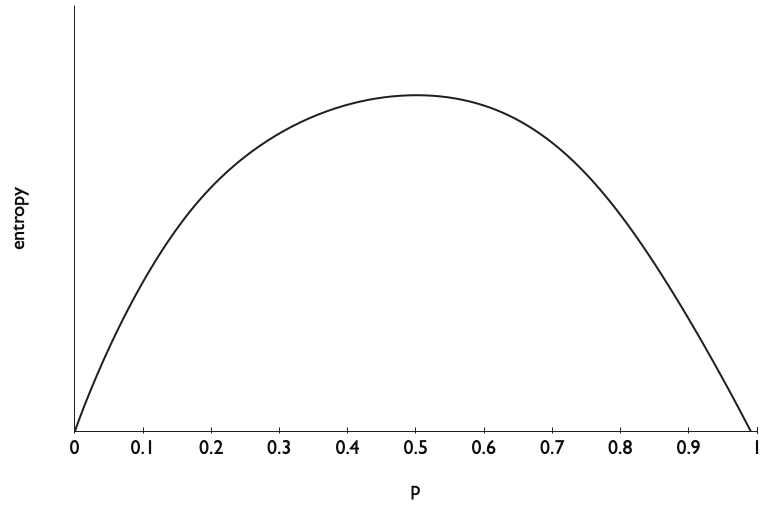
\includegraphics[height=2in]{MyGraph5.eps}
\caption[Entropy]{Entropy as a function of $\hat \pi_1$ when $\pi_1 = .5$.}\label{fig_entropy_I2}
\end{figure}

\begin{example}
Take an $n$-sided possibly unfair die with  a probability distribution $\{p_i\}_{i=1}^n$.
The die is fair if $p_i = \frac{1}{n} \forall i$.  Among all dies, a fair die  maximizes entropy.  For a fair die,
entropy equals $H(p) = - n^{-1} \sum_i \log \left( \frac{1}{n} \right) = \log(n)$.
\end{example}

\begin{remark}
To specify the expected number of bits needed to isolate the outcome of one roll of a fair $n$-sided die requires $\log_2 (n)$ bits of information.  For example,
if $n=2$, $\log_2(2) =1$.  For $n=3$, $\log_2(3) = 1.585$.
\end{remark}



\subsection{Mathematical features of entropy}

For a discrete random variable with probability vector $p$, entropy $H(p)$ is
a function that satisfies
\begin{enumerate}
\item $H$ is {\em continuous}.
\item $H$ is {\em symmetric}: $H(p_1, p_2, \ldots, p_n) = H(p_{r_1}, \ldots, H(p_{r_n})$ for any
permutation $r_1, \ldots, r_n$ of $1,\ldots, n$.
\item A uniform distribution maximizes $H(p)$:
$ H(p_1, \ldots, p_n) \leq H(\frac{1}{n}, \ldots, \frac{1}{n}) .$
\item Maximum entropy increases with the number of states:
$ H(\frac{1}{n}, \ldots, \frac{1}{n} ) \leq H(\frac{1}{n+1}) , \ldots, \frac{1}{n+1})$.
\item Entropy is not affected by events zero probability.
\end{enumerate}

\subsection{Conditional entropy}

Let $(X,Y)$ be a bivariate discrete random vector with  outcomes $x_1, \ldots, x_n$ and $y_1, \ldots, y_m$, respectively,
occurring with probability density $p(x_i, y_i)$.  The conditional entropy $H(X| Y)$ is
defined as
\begin{equation}\label{Shannon2}
H(X | Y) = \sum_{i,j} p(x_i,y_j) \log \frac{p(y_j)}{p(x_i,y_j)}.
\end{equation}
Here $\frac{p(y_j)}{p(x_i,y_j)}$, the reciprocal of the conditional probability of $x_i$ given $y_j$, can be defined
as the conditional surprisal.

\subsection{Maximum conditional entropy and independence}

Let $m=n$ and $[x_1, \ldots, x_n ] = [y_1, \ldots, y_n]$.  Let $\sum_j p(x_i,y_j) = \sum_j p(x_j, y_i) $ for all $i$,
so that the marginal distributions of $x$ and $y$ are identical.  Thus, $x$ and $y$ are identically distributed, but they
are not necessarily independent.
Consider the following:
\begin{problem}\label{Shannon_indep}
Choose the joint distribution  $p(x_i,y_j)$ to maximize  conditional entropy
(\ref{Shannon2}) subject to the restriction that  $x$ and $y$ are identically distributed.  The conditional-
entropy-maximizing  $p(x_i,y_j)$ sets
\[ \frac{p(x_i,y_j)}{p(y_j)} = \sum_j p(x_i, y_j) = p(x_i)  \forall i .\]
Thus, among all joint distributions with identical marginal distributions,
 the conditional entropy maximizing joint distribution makes $x$ and $y$ be
independent.
\end{problem}


\subsection{Thermodynamics}
Gibbs defined entropy as
\begin{equation} \label{Gibbs}
S= - k_B \sum_i p_i  \log p_i
\end{equation}
where $p_i$ is the probability of a micro state and $k_B$ is Boltzmann's constant.\footnote{The Boltzmann constant $k_b$ relates energy at the micro  particle level with the temperature observed at the macro level. It equals what is called a gas constant  divided by an Avogadro constant.}
The second law of thermodynamics states that entropy of a physical system increases until (\ref{Gibbs}) attains its maximum.




\subsection{Kullback Leibler divergence a.k.a. relative entropy}

Let $X$ be a discrete state space $x_1, \ldots, x_n$ and let $p$ and $q$ be  two discrete probability
distributions on $X$.  Assume that $\frac{p_i}{q_t} \in (0,\infty)$ for all $i$ for which $p_i >0$.
Then the Kullback-Leibler measure of divergence, also called {\em relative entropy},
is defined as
\begin{equation}\label{Shannon3}
D(p|q) = \sum_i p_i \log \left(\frac{p_i}{q_i}\right) = \sum_i q_i \left( \frac{p_i}{q_i}\right) \log\left( \frac{p_i}{q_i}\right) .
\end{equation}

Evidently,
\begin{eqnarray}
D(p|q) &=& - \sum_i p_i \log q_i + \sum_i p_i \log p_i \cr
  & = & H(p,q) - H(p)   ,\end{eqnarray}
where $H(p,q) = \sum_i p_i \log   q_i$ is the cross-entropy.

It is easy to verify, as we have in section \ref{sec:entropynonneg}, that $
D(p|q) \geq 0$ and that $D(p|q) = 0$ implies that $p_i = q_i$ when $q_i >0$.

\subsection{Continuous distributions}

For a continuous random variable, Kullback-Leibler divergence between two densities $p$ and $q$ is defined as
\[D(p|q) = \int p(x) \log \left(\frac{p(x)}{q(x)} \right) d \, x .\]

\begin{example}\label{KL_Gaussian_example}
Let  $N_0 = {\mathcal N}(\mu_0,\Sigma_0)$ and $N_1={\mathcal N}(\mu_1, \Sigma_1)$ be two multivariate Gaussian
distributions. Then
\begin{equation}\label{Shannon5}
D(N_0|N_1) = \frac{1}{2} \left(\mathrm {trace} (\Sigma_1^{-1} \Sigma_0)
+ (\mu_1 -\mu_0)' \Sigma_1^{-1} (\mu_1 - \mu_0) - \log\left( \frac{ \mathrm {det }\Sigma_0 }{\mathrm {det}\Sigma_1}\right)
   - k \right).
\end{equation}
\end{example}


\subsection{Backus-Chernov-Zin entropy}
After flipping signs, \citet{BCZ2012} use Kullback-Leibler relative entropy as a measure of volatility of stochastic discount factors that they
assert is useful for characterizing features of both the data and various theoretical models of stochastic discount factors.

Where $p_{t+1}$ is the physical or `true' measure, $p_{t+1}^*$ is the risk-neutral measure, and $E_t$ denotes conditional
expectation under the $p_{t+1}$ measure,
 \citet{BCZ2012}
 define entropy as
\begin{equation} \label{eqn:BCZ1}
L_t (p_{t+1}^*/p_{t+1}) = - E_t \log( p_{t+1}^*/p_{t+1}).
\end{equation}
Evidently, by virtue of the minus sign in (\ref{eqn:BCZ1}),
\begin{equation} \label{eqn:BCZ2}
L_t (p_{t+1}^*/p_{t+1})  = D_{KL,t}( p_{t+1}^*|p_{t+1}),
\end{equation}
where $D_{KL,t}$ denotes conditional relative entropy.

Let $m_{t+1}$ be a stochastic discount factor, $r_{t+1}$ a gross one-period return on a risky
security, and $(r_{t+1}^1)^{-1}\equiv q_t^1 = E_t m_{t+1}$ be the reciprocal of a risk-free one-period gross rate of return.
Then
\[ E_t (m_{t+1} r_{t+1}) = 1 \]
\citeauthor{BCZ2012} note that a stochastic discount factor satisfies
\[ m_{t+1} = q_t^1 p_{t+1}^*/p_{t+1} .\]
They derive the following {\em entropy bound}
\begin{equation}
E L_t (m_{t+1}) \geq E (\log r_{t+1} - \log r_{t+1}^1 )
\end{equation}
which they propose as a complement to the Hansen-Jagannathan bound.

\subsection{Wiener-Kolmogorov prediction error formula as entropy}

Let $\{x_t\}_{t=-\infty}^\infty$ be a covariance stationary stochastic process with
mean zero and spectral density $S_x(\omega)$. The variance of $x$ is
\[ \sigma_x^2 =\left( \frac{1}{2\pi}\right) \int_{-\pi}^\pi  S_x (\omega) d \omega . \]
The Wiener-Kolmogorov formula for the one-period ahead prediction error is
\begin{equation}\label{Shannon6}
\sigma_\epsilon^2 = \exp\left[\left( \frac{1}{2\pi}\right) \int_{-\pi}^\pi \log S_x (\omega) d \omega \right].
\end{equation}
Occasionally the logarithm of  the one-step-ahead prediction error $\sigma_\epsilon^2$
is called entropy because it measures unpredictability.

Consider the following problem  reminiscent of problem \ref{Shannon_indep}.

\begin{problem}\label{prob:Wiener_Kolm}
Among all covariance stationary univariate processes with unconditional variance $\sigma_x^2$, find a process with maximal
one-step-ahead prediction error.
\end{problem}

\noindent The maximizer of  problem \ref{prob:Wiener_Kolm} is  a process with spectral density
\[ S_x(\omega) = 2 \pi \sigma_x^2.\]
Thus,  among
all univariate covariance stationary processes with variance $\sigma_x^2$, a process with a flat spectral density is the most uncertain, in the sense of one-step-ahead prediction error variance.  This no-patterns-across-time outcome for a temporally dependent process resembles the no-pattern-across-states outcome for the static entropy maximizing coin or die  in the classic information theoretic
analysis described in section \ref{sec:Shannon1}.

\subsection{Multivariate process}

Let $y_t$ be an $n \times 1$ covariance stationary stochastic process with mean $0$ with
matrix covariogram $C_y(j) = E y_t y_{t-j}' $ and spectral density matrix
\[ S_y(\omega) = \sum_{j=-\infty}^\infty e^{- i \omega j} C_y(j), \omega \in [-\pi, \pi].  \]
Let
\[ y_t = D(L) \epsilon_t  \equiv \sum_{j=0}^\infty D_j \epsilon_t \]
be a Wold representation for $y$, where $D(0)\epsilon_t$ is a
vector of one-step-ahead errors in predicting $y_t$ conditional on the infinite history $y^{t-1} = [y_{t-1}, y_{t-2}, \ldots ]$ and
$\epsilon_t$ is an $n\times 1$ vector of serially uncorrelated random disturbances with mean zero and identity contemporaneous
covariance matrix $E \epsilon_t \epsilon_t' = I$.
 Linear-least-squares predictors have one-step-ahead prediction error $D(0)  D(0)'$
  that satisfies
\begin{equation}\label{Shannon2}
\log \det [D(0) D(0)'] = \left(\frac{1}{2 \pi} \right) \int_{-\pi}^\pi \log \det [S_y(\omega)] d \omega.
\end{equation}
Being a  measure of the unpredictability of an $n \times 1$ vector covariance stationary  stochastic process,
 he left side of  \eqref{Shannon2} is sometimes called entropy.
\subsection{Frequency domain robust control}

\citet[ch.~8]{HSrobustnessmonograph} adapt work in the control theory literature to define a
frequency domain {\em entropy} criterion for  robust control as
\begin{equation}\label{Shannon21}
\int_\Gamma \log \det [ \theta I - G_F(\zeta)' G_F(\zeta) ] d \lambda(\zeta) ,
\end{equation}
where $\theta \in (\underline \theta, +\infty)$ is a positive robustness parameter and $G_F(\zeta)$ is a $\zeta$-transform of the
objective function.  Hansen and Sargent show that (\ref{Shannon21}) can be represented as
\begin{equation}\label{Shannon22}
\log \det [ D(0)' D(0)] = \int_\Gamma \log \det [ \theta I - G_F(\zeta)' G_F(\zeta) ] d \lambda(\zeta) ,
\end{equation}
for an appropriate covariance stationary stochastic process derived from $\theta, G_F(\zeta)$. This explains the
moniker `maximum entropy' robust control for decision rules $F$ designed to maximize (\ref{Shannon21}).




\subsection{Relative entropy for a continuous random variable\label{sec:entropynonneg}}

Let $x$ be  a continuous random variable with density $\phi(x)$, and let $g(x) $ be a nonnegative random variable satisfying $\int g(x) \phi(x) dx =1$.
The relative entropy of the distorted density $\hat \phi(x) = g(x) \phi(x)$  is defined
as
\[ \textrm{ent}(g) = \int g(x) \log g(x) \phi(x) d x .\]
Figure \ref{fig_glogg3} plots the functions $g \log g$ and $g -1$
over the interval $g \geq 0$.   That relative entropy $\textrm{ent}(g) \geq 0$ can be established by noting (a) that  $g \log g \geq g-1$ %(see figure \ref{fig_glogg3})
 and (b) that under $\phi$, $E g =1$.
%Because $g \log g \geq 1$, $E g \log g \geq 0$.

Figures \ref{fig_glogg1} and \ref{fig_glogg2} display aspects of relative entropy visually for a continuous random variable $x$ for
two densities with likelihood ratio $g \geq 0$.  Where the numerator density is ${\mathcal N}(0,1)$, for two denominator  Gaussian densities ${\mathcal N}(0,1.5)$ and ${\mathcal N}(0,.95)$, respectively, figures
\ref{fig_glogg1} and \ref{fig_glogg2} display the functions  $g \log g$ and $g -1$ as functions of $x$.  %Because $g \log g \geq g -1$ and because
%$E g =1$ under the density in the denominator, it follows that $E g \log g \geq 0$.


\begin{figure}[htp]
\centering
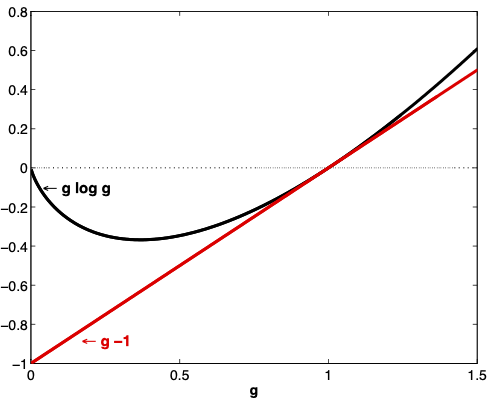
\includegraphics[height=2in]{entropy_glogg.eps}
\caption[$g \log g$ for $g \geq 0$]{The function $g \log g$ for $g \geq 0$. For a random variable $g$ with $E g =1$, $E g \log g \geq 0$.}\label{fig_glogg3}
\end{figure}

\begin{figure}[htp]
\centering
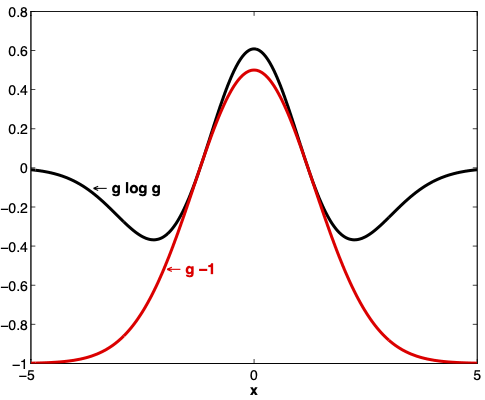
\includegraphics[height=2in]{entropy_1_over_15.eps}
\caption[$g \log g$ and $g-1$]{Graphs of $g \log g$ and $g-1$ where  $g$ is the ratio of the density of a ${\mathcal N}(0,1)$ random variable to the density of a ${\mathcal N}(0,1.5)$ random variable.
Under the ${\mathcal N}(0,1.5)$ density, $E g =1$.}\label{fig_glogg1}
\end{figure}

\begin{figure}[htp]
\centering
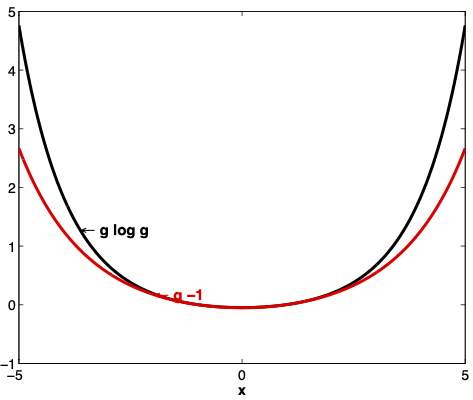
\includegraphics[height=2in]{entropy_1_over_95.eps}
\caption[$g \log g$ and $g-1$ again]{Graphs of $g \log g$ and $g-1$ where $g$ is the ratio of the density of a ${\mathcal N}(0,1)$ random variable to the density of a ${\mathcal N}(0,.95)$ random variable.
Under the ${\mathcal N}(0,.95)$ density, $E g =1$.}\label{fig_glogg2}
\end{figure}


\end{subappendices}